\documentclass[12pt]{article}
\usepackage[letterpaper, margin=0.25in]{geometry}
\usepackage{blindtext}
\usepackage[utf8]{inputenc}
\usepackage{graphicx} 
\usepackage{float} 
\usepackage{karnaugh-map}
\usepackage{rotating}
\usepackage{pdflscape}
\usepackage{caption}
\usepackage{booktabs}
\usepackage{subcaption}
\usepackage{placeins}
\usepackage{gensymb}
\usepackage{siunitx}
\usepackage{bigstrut}
\usepackage{multicol}
\usepackage{multirow}
\usepackage{color, colortbl}
\graphicspath{ {./Figures} }

\usepackage[compact]{titlesec}
\titlespacing{\section}{0pt}{*0}{*0}
\titlespacing{\subsection}{2pt}{*0}{*0}


\newcommand{\foo}{\hspace{-2.3pt}$\bullet$ \hspace{5pt}}
\newcommand{\ts}{\textsuperscript}

\begin{document}
\title{\textbf{Preliminary Sensor Selection}}
\author{
  Alan Harris\\
  250901911
  \and
  Robert Potra\\
  250914807
  \and
  Andrew Randell\\
  250911270
  \and
  Kevin Wang\\
  250908180
}
\date{\today}
\maketitle

\setcounter{page}{1}

\vspace*{-\baselineskip}

\section{Introduction}

To perform the task autonomously the robot requires information about its surroundings. Sensors are used to relay information about the changing environment to help the robot make decisions. The entire problem was divided into tasks that require different sensing capabilities, and therefore, the tasks include tracking the robot's position relative to the perimeter, detecting the tesseract, detecting the pyramid, and tracking the robot's position for outdoor applications. Key requirements for each task were outlined in Report 1.

\section{Wall Following Requirement}
\subsection{Concept Generation}

The autonomous system will need to follow the perimeter wall of the power plant. The distance at which the system follows the wall will need to be precisely maintained at a constant value of 1.5 meters $\pm$ 5\%. With these requirements, various concepts were generated.

\begin{itemize}
\setlength\itemsep{-0.5em}
\item Rotary Encoders can be used to track movement of wheels and adjust as needed.
\item LVDTs, Linear Potentiometers, ultrasonic sensors, and infrared sensors can be used at forward and aft locations of the autonomous system. The difference between the two readings will determine if the system is parallel with the wall and the distance the system is from the wall.
\item
Computer Vision using wide field of views cameras could be used to pick out objects in the surrounding area. Cameras could be used to find and maintain a parallel distance with the wall. LIDAR can be used in conjunction with computer vision with a more precise distance information. SONAR and RADAR display objects in the immediate radius of the system. These advanced systems can be mounted in a high location on top of the system to give the system accurate position data.
\item
GNSS systems can be implemented to give the system latitude, longitude, and altitude coordinates. A 2-dimensional map can be stored in memory which the system will used to navigate.
\end{itemize}


\vspace*{-\baselineskip}
% Table generated by Excel2LaTeX from sheet 'Requirements from Google Doc'
\begin{table}[htbp]
  \centering
  \caption{Wall Following Sensor Requirements}
    \begin{tabular}{c|p{10em}|p{29.72em}}
    \multicolumn{1}{p{6.9em}|}{\textbf{Variable}} & \textbf{Requirement} & \textbf{Reasoning} \bigstrut[b]\\
\hline
    \multicolumn{1}{c|}{\multirow{3}[1]{*}{Linear Distance}} & Range: 0.5m-3.0m & Prevent the robot from colliding with surrounding \bigstrut[t]\\
          & Response Time: 0.1s & \multicolumn{1}{l}{Ensure the robot can respond quickly enough to avoid collisions } \\
          & Sample Rate: $>$ 10 Hz & Ensure the system receives sensor data at an acceptable rate \\
    \end{tabular}%
  \label{tab:addlabel}%
\end{table}%





\subsection{Concept Selection}

\begin{itemize}
\setlength\itemsep{-0.5em}
\item The LVDT, Potentiometer, and Limit Switch were eliminated first because they rely on physical contact with the surroundings. These are not feasible as contacting the wall will quickly wear the sensors. In addition, the range is far too small, and should not be limited to a simple binary contact.

\item Encoders on the wheels were ruled out as there is a strong dependence on full traction of the wheels. The slightest loss of grip will throw off the sensors entirely, and will give inaccurate readings.

\item Capacitive Sensors were eliminated because the scale of the measurements is far too small for the size of the robot. Considering that the wall area is quite large, a capacitive sensor will not be able to provide the range necessary to accurately detect local position.

\item Ultrasonic sensors provide a contactless solution that provides decent accuracy and repeatability. When the robot is close to a perimeter wall, they will be sufficient for navigation.

\item GNSS struggles to provide coordinates that have greater accuracy than +- 5 meters. Due to this, GNSS is acceptable for approximate positioning, such as locating a constant home location or for locating known coordinates of areas of rough terrain. 
\end{itemize}

\subsection{Concept Choice}
For local positioning, six pairs ultrasonic sensors will be used on the robot: two pairs of sensors will be on the left and right sides, and a single pair of sensors will be on the front and back. Alignment and distance from the perimeter wall will be determined from this sensor setup. This setup also provides redundancy if some of the sensors fail. The applicable pairs of sensors will have plausibility checks to determine if the system is functioning properly. If the system fails plausibility checks, the robot will shut down and require human intervention.

For global positioning, a GNSS module will be used to provide latitude and longitude coordinates. When the system is initially called upon to initiate work, the GNSS will guide the robot to its home location. From its home location, the robot will be able to rely upon the ultrasonic sensors to navigate along the perimeter wall. The GNSS will also play a role in pyramid location which will be discussed later. 


\subsection{Concept Model}
\begin{figure}[htb!]
\begin{center}
\caption{Ultrasonic Sensor Model}
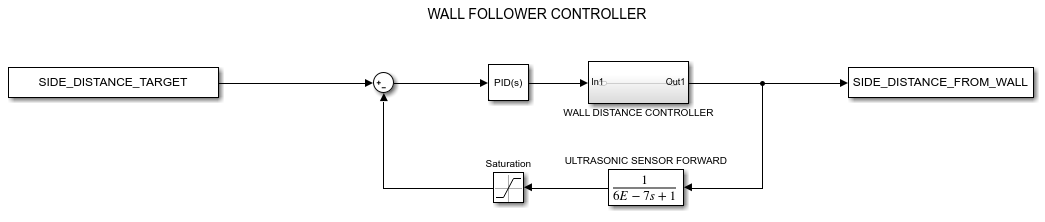
\includegraphics[scale=0.6]{Figures/simulink_ultrasonic}
\end{center}
\end{figure}
\FloatBarrier

\vspace*{-\baselineskip}
\section{Tesseract Detection}
\subsection{Concept Generation}
\begin{itemize}
\item Since the tesseract emits a strong magnetic field. A magnetic sensor mounted on the tesseract intake can be used to detect its presence. 1-axis hall-effect sensors could be used, or a 3-axis magnetometer could be used by taking the magnitude of the 3 axes.

\item The system could sweep the entire perimeter and catch the tesseract in a chute which could trip a limit switch.

\item A limit switch could be used on the tesseract intake which would trigger when the tesseract is within grabbing distance. A magnetic Reed switch could be used as an alternative to the limit switch.
\end{itemize}

% Table generated by Excel2LaTeX from sheet 'Requirements from Google Doc'
\begin{table}[htbp]
  \centering
  \caption{Tesseract Sensor Detection Requirements}
    \begin{tabular}{c|p{11.5em}|p{29.89em}}
    \multicolumn{1}{p{5.5em}|}{\textbf{Variable}} & \textbf{Requirement} & \textbf{Reasoning} \bigstrut[b]\\
    \hline
    Magnetic & Linearity Error: $<$ 2\% & Accurately detect the location of the magnetic field from tesseract \bigstrut[t]\\
    Field  & Low Reliability Error & Consistently and accurately locate the position of the tesseract \\
    Strength & Resolution: $<$ 1 mG & Detect small changes in magnetic field to move toward tesseract \\
    \end{tabular}%
  \label{tab:addlabel}%
\end{table}%


\subsection{Concept Selection}
The Hall Effect sensor is a standard sensor which excels in proximity sensing, position, speed detection and current sensing applications. However, hall effect sensor has a lower measuring accuracy and sensitivity—which is an important factor for improving the robot’s functionality—and the output signal tends to drift. For these reasons, it is unacceptable as a sensor to find the tesseract.
The reed switch was also an unideal option, as it relies on physical contact. This means that the range and sensitivity are extremely low, as well as only returning a binary value. Additionally, the life expectancy is lower due to the mechanical nature of the sensor.
A vector-based magnetometer is the best sensor for finding the tesseract. This sensor delivers a high level of sensitivity and dynamic range. Additionally, noise and temperature drift are kept low. 

\subsection{Concept Choice}
A contactless method of detecting the tesseract cube is prefered.as this reduces wear and tear on the system and can increase the operating speed. Magnetometers provide a solid contactless method of measuring the magnetic field at a given point. Since the magnetic field of the Tesseract is approximately 800 mT, which is comparable to an MRI machine, the magnetometer should not have any difficulty distinguishing between the earth’s magnetic field or other nearby magnetic fields such as motors.
\subsection{Concept Model}\begin{figure}[htb!]
\begin{center}
\caption{Infrared Sensor Model}
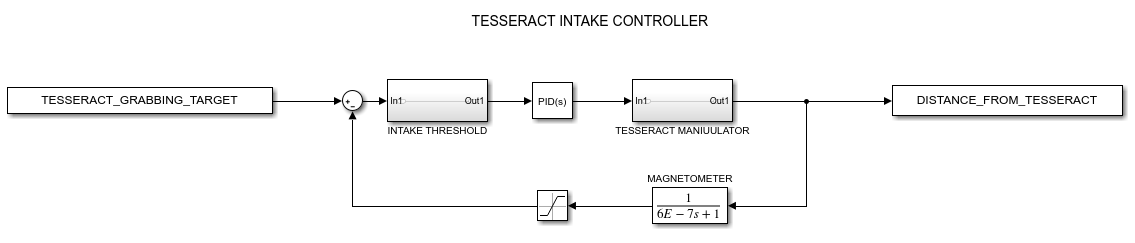
\includegraphics[scale=0.6]{Figures/simulink_tesseract}
\end{center}
\end{figure}
\FloatBarrier

\section{Pyramid Detection}
\subsection{Concept Generation}
\begin{itemize}
\setlength\itemsep{-0.5em}
\item Since the pyramids are massive, LIDAR, SONAR, RADAR or Computer Vision data could be analyzed for readings that have the shape of a pyramid.

\item Infrared sensors could be used to receive a signal from the pyramid’s infrared blaster.
\end{itemize}

% Table generated by Excel2LaTeX from sheet 'Requirements from Google Doc'
\begin{table}[htbp]
  \centering
  \caption{Add caption}
    \begin{tabular}{c|p{9.89em}|p{28.165em}}
    \multicolumn{1}{p{7.445em}|}{\textbf{Variable}} & \textbf{Requirement} & \textbf{Reasoning} \bigstrut[b]\\
    \hline
    \multicolumn{1}{p{7.445em}|}{Presence and} & Rise Time: $<$ 0.05s & Adjust robot’s direction of travel toward pyramid IR light quickly \bigstrut[t]\\
    Direction of & Field of View: $>$ 90 \degree & Increase chances of exposure to pyramid’s IR light \\
    IR Light & Sample Rate: $>$ 10 Hz & Provide system at a sufficiently fast rate \\
    \end{tabular}%
  \label{tab:addlabel}%
\end{table}%




\subsection{Concept Selection}
In order to decode the infrared (IR) signal sent by the pyramid, an IR sensor will be used.  IR sensors excels in this application because of its ability pick up signals in a large area. This is a useful quality as it makes pyramid detection easier, especially used in conjunction with  GNSS. IR sensors also have high repeatability and provide good stability over time. An important note for this sensor is that the transmitter and receiver must be in line of sight (LOS). The final design of the robot must ensure that the IR sensor is in LOS with the transmitter within the pyramid. 

\subsection{Concept Choice}
An infrared sensor combined with the GNSS coordinates will be used to determine the location of the pyramid. Because the range of the IR sensors is fairly limited, it cannot solely be relied upon for pyramid positioning. Locating the pyramid will consists of a series of 360-degree IR scans on a grid of points on the map. The map of the power plant will be divided into a grid of squares with dimensions of 5m x 5m. At each point on this grid, the robot will execute a 360-degree scan. If the robot has completed the task before, the robot will have the coordinates of the pyramid location stored in memory from the last cycle. If this is the case, it will rely upon GNSS to determine the rough location of the pyramid. 


\subsection{Concept Model}
\begin{figure}[htb!]
\begin{center}
\caption{Infrared Sensor Model}
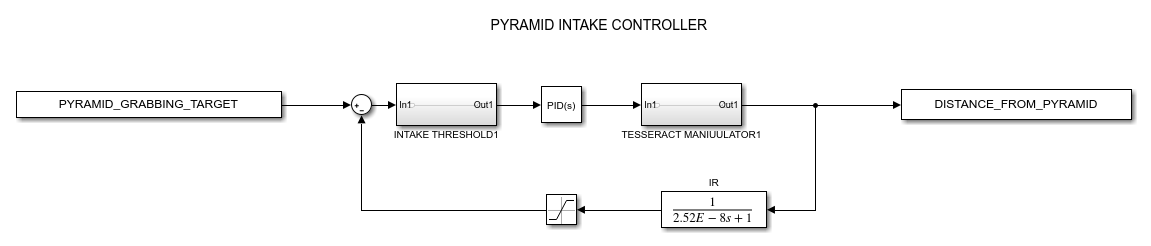
\includegraphics[scale=0.6]{Figures/simulink_pyramid}
\end{center}
\end{figure}
\FloatBarrier

\section{Project Timeline}
Our team was able to follow the project timeline specified in our previous report. As a result, we have decided to keep the same timeline, with updated dates. Should our team encounter difficulty following the timeline, updates will be made in future reports to reflect the current state of work.\\
\begin{flushleft}

\textit{Week of:}

\begin{tabular}{l | l} 
\textbf{Feb. 18} &\textbf{Research Applicable Actuators}\\
 & $\bullet$ Restate and redefine actuator specifications\\
  & $\bullet$ Identify possible actuator options based on previous concepts\\
  
\textbf{Feb. 25} & \textbf{Continue Actuator Design}\\
 & $\bullet$ Concept generation using possible actuator options\\
  & $\bullet$ Refine logic connecting the sensor data to actuator actions\\
  
\textbf{Mar. 04} & \textbf{Finalize Actuator Simulations}\\
 & $\bullet$ Perform actuator simulations using Simulink\\
 & $\bullet$ Begin preparing report for step 3 deliverable\\
 & $\bullet$ Perform concept selection using actuator simulation results and analysis\\
 
\textbf{Mar. 11} &\textbf{Preliminary Actuator Selection Deliverable: Step 3 Due Mar. 15\ts{th}}\\
 & $\bullet$ Continue preparing and finalize report step 3 deliverable\\
 
\textbf{Mar. 18} & \textbf{Evaluate Sensor and Actuators}\\
 & $\bullet$ Evaluate the proposed system of sensors and actuators\\
  & $\bullet$ Create a kinematic system model and perform analysis using Solidworks\\
  
\textbf{Mar. 25} & \textbf{Obtain Feedback and Iterate}\\
  & $\bullet$ Identify possible problems with the proposed system of sensors and actuators\\
  & $\bullet$ Refine analysis for the transducers, control device, kinematics, and power supply\\
  
\textbf{Apr. 01} & \textbf{Finalize Final Simulations and Report: Step 4 Due Apr. 5\ts{th}}\\
 & $\bullet$ Continue preparing final report for step 4 deliverable\\

\end{tabular}
\end{flushleft}

\begin{figure}[htb!]
% Table generated by Excel2LaTeX from sheet 'GONOGO'
\begin{table}[H]
  \centering
  \caption{GO/NO GO Table (\textit{"1" = GO, " " = NO GO)}}
    \begin{tabular}{p{15.645em}|c|c|c|c|c|c|c|c|c|c|c}
    \multicolumn{1}{r}{} & \multicolumn{1}{c}{\begin{sideways}\textbf{Range}\end{sideways}} & \multicolumn{1}{c}{\begin{sideways}\textbf{Accuracy}\end{sideways}} & \multicolumn{1}{c}{\begin{sideways}\textbf{Sensitivity}\end{sideways}} & \multicolumn{1}{c}{\begin{sideways}\textbf{Sample Rate}\end{sideways}} & \multicolumn{1}{c}{\begin{sideways}\textbf{Stability}\end{sideways}} & \multicolumn{1}{c}{\begin{sideways}\textbf{Repeatability}\end{sideways}} & \multicolumn{1}{c}{\begin{sideways}\textbf{Linearity}\end{sideways}} & \multicolumn{1}{c}{\begin{sideways}\textbf{Ease of Use}\end{sideways}} & \multicolumn{1}{c}{\begin{sideways}\textbf{Elegance}\end{sideways}} & \multicolumn{1}{c}{\begin{sideways}\textbf{Long Life}\end{sideways}} & \begin{sideways}\textbf{Non-Contact}\end{sideways} \\
    \midrule
    \textbf{Local Position} &       &       &       &       &       &       &       &       &       &       &  \\
    LVDT (probes) &       & 1     & 1     & 1     & 1     & 1     & 1     &       &       & 1     &  \\
\rowcolor{green}    Ultrasonic & 1     & 1     &       & 1     & 1     & 1     & 1     & 1     & 1     & 1     & 1 \\
    Potentiometer (probes) &       & 1     & 1     & 1     & 1     & 1     & 1     &       &       &       &  \\
    Limit Switch (bump into walls) &       &       &       &       &       & 1     &       & 1     &       &       &  \\
    Capacitive &       &       &       & 1     &       &       &       &       &       & 1     & 1 \\
    Encoders (on wheels) & 1     &       &       & 1     &       &       & 1     & 1     & 1     & 1     & 1 \\
    \multicolumn{1}{r|}{} &       &       &       &       &       &       &       &       &       &       &  \\
    \midrule
    \textbf{Global Position} &       &       &       &       &       &       &       &       &       &       &  \\
\rowcolor{green}    GNSS  & 1     & 1     &       &       &       &       & 1     & 1     & 1     & 1     & 1 \\
    RADAR & 1     & 1     & 1     &       & 1     & 1     & 1     &       & 1     & 1     & 1 \\
    SONAR &       &       &       &       &       & 1     & 1     &       & 1     & 1     & 1 \\
\rowcolor{green}    LIDAR & 1     & 1     & 1     & 1     & 1     & 1     & 1     &       & 1     & 1     & 1 \\
    Computer Vision & 1     & 1     & 1     & 1     & 1     & 1     & 1     &       & 1     & 1     & 1 \\
    \multicolumn{1}{r|}{} &       &       &       &       &       &       &       &       &       &       &  \\
    \midrule
    \textbf{Tesseract Detection} &       &       &       &       &       &       &       &       &       &       &  \\
    Hall Effect &       & 1     &       & 1     &       &       & 1     & 1     & 1     & 1     & 1 \\
\rowcolor{green}    Magnetometer & 1     & 1     & 1     & 1     &       & 1     & 1     & 1     & 1     & 1     & 1 \\
    Reed Switch &       &       &       &       &       & 1     &       &       &       &       & 1 \\
    Computer Vision & 1     &       &       &       &       &       &       &       & 1     & 1     & 1 \\
    \multicolumn{1}{r|}{} &       &       &       &       &       &       &       &       &       &       &  \\
    \midrule
    \textbf{Pyramid Detection} &       &       &       &       &       &       &       &       &       &       &  \\
\rowcolor{green}    IR Receiver & 1     & 1     &       & 1     &       &       & 1     & 1     & 1     & 1     & 1 \\
    Computer Vision & 1     &       &       &       &       &       &       &       & 1     & 1     & 1 \\
    \end{tabular}%
  \label{tab:addlabel}%
\end{table}%
\end{figure}
\FloatBarrier





\end{document}